\section{Threads}
Schnellere Programme:
\begin{itemize}[itemsep=0em, parsep=0pt]
    \item Aufteilen einer Datenmenge in mehrere Teile, um parallel zu arbeiten
    \item Teilresultate nach Verarbeitung zusammenführen
    \item Bsp.: Sortierverfahren, Komprimierung, Bildverarbeitung
\end{itemize}
Einfachere Programme:
\begin{itemize}[itemsep=0em, parsep=0pt]
    \item Gleichzeitig oder verzahnt ausführbare Abläufe
    \item Bsp.: Layout, Speichern im Hintergrund
\end{itemize}
Multi-Core-Prozessoren können mehrere Threads parallel ausführen, für jeden Core zwei Threads.

\subsection{JVM Thread Modell}
Java ist ein Single Process System. JVM erzeugt beim Aufstarten einen Thread, welcher \verb|main()| aufruft. Der Programmierer, Subsysteme oder das 
Laufzeitsystem können ebenfalls Threads starten.

Die JVM läuft, solange Threads laufen, ausser wenn Threads als \textit{Daemon} markiert sind (z.B. Garabge Collector). JVM wartet nicht auf Daemon Threads, 
diese werden bei JVM-Ende unkontrollliert abgebrochen.

\subsubsection{Runnable Interface}

\begin{minipage}{0.48\columnwidth}
    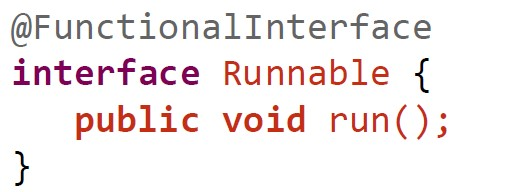
\includegraphics[width=\linewidth]{pictures/runnable-interface.jpg}
\end{minipage}
\hfill
\begin{minipage}{0.48\columnwidth}
    Kann auch als Lambda übergeben werden:\\
    
\includegraphics[width=\linewidth]{pictures/runnable-lambda.jpg}
\end{minipage}
Funktionsschnittstelle eines Threads, sie wird beim Starten des Threads durch die JVM gerufen.

\subsubsection{Start und Ende}
Ein Thread wird nach \verb|start()| ausgeführt (über \verb|run()| des \verb|Runnable|-Interfaces):\\
\lstinputlisting{code/thread.java}

Der Thread endet beim Verlassen von \verb|run|, z.B. durch Ende der MEthode, Return Statemnt oder unbeh. Exception

\subsection{Multi-Thread Beispiel}
\lstinputlisting{code/Demo02MultiThread.java}

\subsection{Alternative Implementationen}
\subsubsection{Explizit}
\lstinputlisting{code/MyRunnable.java}

\subsubsection{Sub-Klasse von Thread}
\lstinputlisting{code/SimpleThread.java}

% \subsection{Ablaufdefinitionen}
% \subsubsection{join()}
% 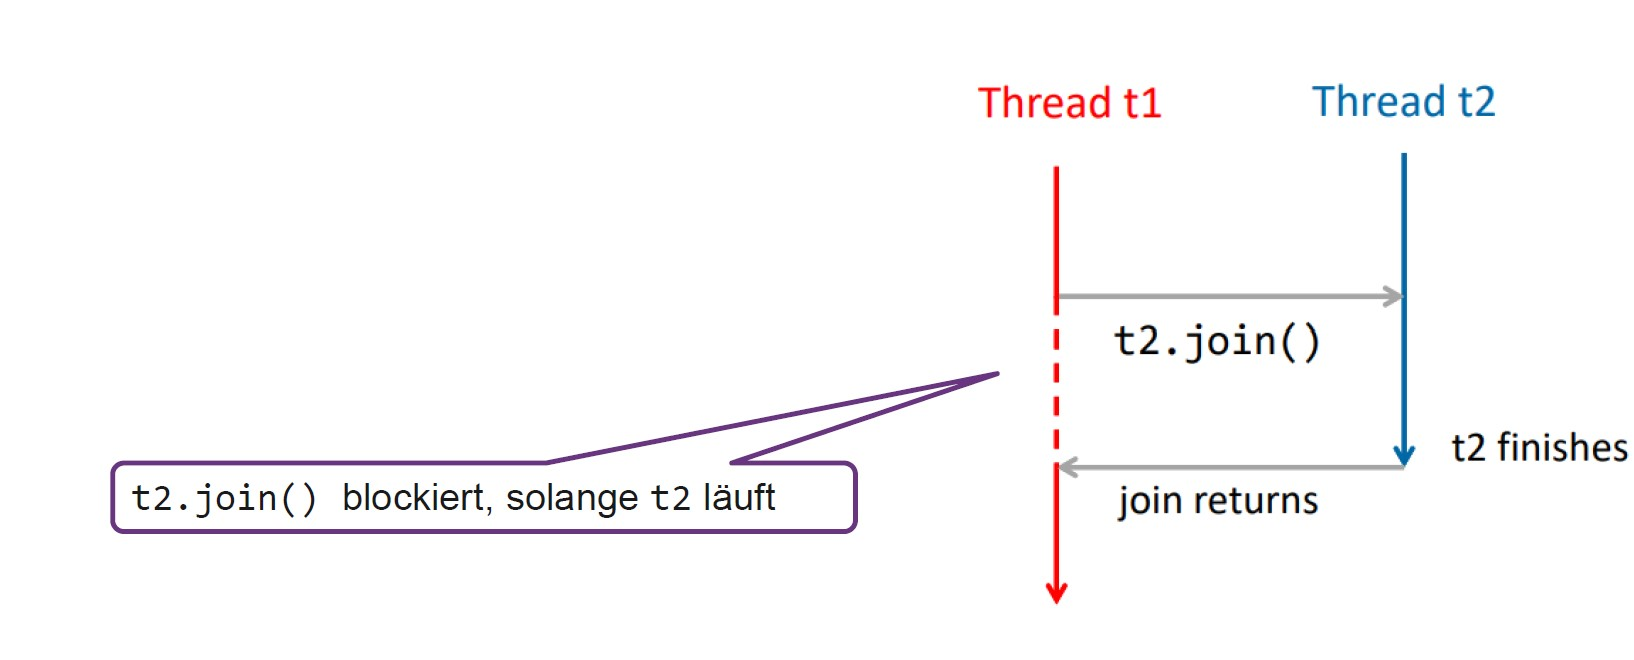
\includegraphics[width=\linewidth]{pictures/thread-join.jpg}

\subsection{Thread-Methoden}

\subsubsection{Thread Passivierung}
\paragraph{Thread.sleep(milliseconds)}
Laufender Thread wird schlafen gelegt

\paragraph{Thread.yield()}
Laufender Thread gibt Prozessor frei und wird wieder ablaufbereit

\subsubsection{InterruptedException}
Mögliche Exception bei blockierenden Aufrufen, z.B. \verb|join(), sleep(), ...|

Threads können von aussen unterbrochen werden: \verb|myThread.interrupt()| $\rightarrow$ bricht \verb|join(), sleep(), ...| ab

\subsubsection{Weitere Methoden}
\verb|static Thread currentThread()| liefert Instanz des Threads \\

\verb|long threadId()| liefert ID des Threads \\

\verb|void setDaemon(boolean on)| Thread als \textit{Daemon} markieren

\subsection{Synchronisation}
Threads teilen sich Adressraum und Heap. Wird auf dasselbe Objekt zugegriffen, muss abgesichert werden.

\verb|synchronized| ist ein Modifier für Methoden, ähnlich wie ein Flag.
\lstinputlisting{code/BankAccount.java}
Nur ein Thread kann eine der \verb|synchronized|-Methoden zur gleichen Zeit in derselben Instanz ausführen